%!TEX root = comps_NKasimov.tex
\chapter{New Volume Penalization Methods}
\label{chapter:3}
\section{Brinkman-like Penalization for Low Fidelity Simulations}
Due to the coarse grid used in Lo-Fi simulations slightly modified BP methods was developed, in order to match drag force that drives particles obtained numerically with experimental results. The idea is to introduce momentum penalization term which is quadratic in velocity
\begin{align}
\frac {\pt \rho u_i}{\pt t} &= RHS - \frac \chi \eta \rho \rbr{u_i - U_i^o}^2.
\end{align}
From one hand, it forces the solution to the proper value at the obstacle boundary even faster than in case of simple BP, on the other hand this expression makes modeling of the penalization easier and flow independent. Namely, 
\begin{align}
F_{drag} &= \int\displaylimits_\Omega \frac 1 \eta \rho \rbr{u - U^o}^2\ dV \sim \int \displaylimits_A \frac 12 \rho C_d \rbr{u - U^o}^2\ dA, \label{eq:lofi-penal}
\end{align}
where $\Omega$ is the volume of the obstacle, and $A$ is largest cross section are across the flow and $\chi$ is dropped since integration is performed only inside of the obstacle. For the sake of simplicity, let us consider uniform flow around triaxial ellipsoid with semi axes $a,b$ and $c$. In that case $\Omega = \pi a b c$ and $A = \pi a b$, under the assumption that flow goes along $c$ semi axis. So, \eqref{eq:lofi-penal} simplifies into
\begin{align}
\frac {\pi a b c}\eta \sim \frac 12 \pi a b\ C_d \implies \eta \sim \frac c{2C_d}
\end{align}

\section{Characteristic Based Volume Penalization}
First VP method used in Hi-Fi simulations was Brinkman Penalization. For testing purposes 1D Riemann problem for Euler equations were solved (see Fig.~\ref{fig:riemann_euler}).
\begin{figure}[h!]
\centering 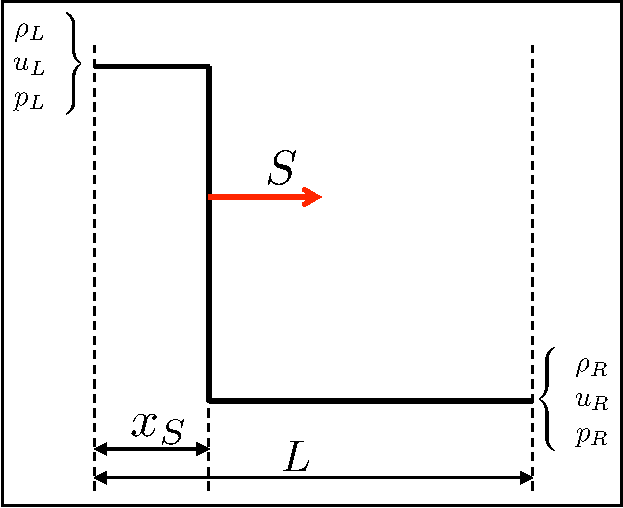
\includegraphics[scale=0.5]{fig/Riemann_Euler.pdf}\\
\caption{Riemann problem set up \label{fig:riemann_euler}}
\end{figure}

To compare results, first, normal self-sustained shock problem was solved with reflection on the right domain boundary. Then right domain was extended and part of the domain was considered as solid obstacle and BP was used to model that solid obstacle/wall. Results revealed that using BP without any modification to supersonic flow leads to significant numerical errors such as phase lag amplitude error, e.g. pressure seepage (see Fig.~\ref{fig:plain_bp}).

In order to overcome deficiencies of BP regarding flow regimes and boundary conditions, new VP method was developed. Let us consider general BC that one wants to mimic at the fluid-solid interface
\begin{align}
\mathcal L \rbr \bullet = f_{boundary},
\end{align}
where $\rbr \bullet$ may stand for any of the integrated variables, and operator $\mathcal L$ can describe either Dirichlet or Neumann boundary conditions, or both. The idea is replace evolution problem under the consideration as follows:
\begin{align}
\frac {\pt \phi}{\pt t} = RHS \longrightarrow \frac {\pt \phi}{\pt t} = RHS - \frac \chi \eta \sbr{\mathcal L \rbr \phi - f_{boundary}}.
\end{align}
Obviously, BP method is a special case of CBVP, when $\mathcal L = \mathds 1$ and $f_{boundary} = U^o$ for velocity or $f_{boundary} = T^o$ for temperature. Let us consider 
